\documentclass{article}

\usepackage{graphicx} %package to manage images
\graphicspath{ {../misc/} }
\usepackage[a4paper, total={6in, 8in}]{geometry}

\begin{document}

\title{Permissionless Escrowed Governance Incentives for Blockchain-based Organizations}

\author{
Joshua Weintraub\thanks{Special thanks to @greenbergz and the team at Redacted Cartel, Ganesh Vanahalli, Vipul Ujawane, and Ryan Tinder for consulting and providing feedback.}
}


\maketitle

\begin{abstract}

This paper attempts to discuss the ways in which current models of DAO governance may be unduly influenced by the existence of malicious incentives for user votes. Over the last several years the rise of Gauge-Proxy token distribution models has resulted to a cottage industry whereby companies connect users wishing to sell their Gauge-Proxy votes to certain pools in exchange for payment in tokens. The voting power of these users however extends far beyond Gauge-Proxy, resulting in unexpected and negative outcomes for DAO governance. Contrary to popular belief, the existence of these incentives is not entirely negative, but must be handled with care to prevent centralized and malicious outcomes. There exists no research attempting to quantify the extend of this problem or design a suitable solution. In this paper I present ERC-6506, a universal standard for enabling DAO voters to solicit incentives for their votes while avoiding negative externalities. Organizing a central location for these activities allows creation of a more efficient marketplace which accrues value to all while preserving decentralization.


\end{abstract}

\tableofcontents



\section{Background}

In August of 2020 decentralized token exchange \emph{Curve Finance} released their Decentralized Autonomous Organization (DAO) alongside its governance token \emph{CRV}. Holders of the CRV token would be responsible for presiding over changes to the Curve-DAO, with number of votes being proportional to amount of vested CRV-tokens. \footnote{Votes are determined not sole by CRV-token, but by amount of CRV tokens locked into Ve-CRV tokens for a predetermined period of time at a linear decay rate. Anyone can lock CRV tokens with longer locking periods meaning higher voting weight}. In addition to the CRV-DAO launch, a new feature was introduced as well, \emph{Gauge Proxy}. This system would determine the inflationary schedule of the CRV token, particularly how new tokens were created and to whom they were distributed to at predetermined intervals.

\subsection{Liquidity Pools}

Curve Finance is a decentalized exchange which utilizes the concept of an "Automated Market Maker". Traditional exchanges, such as the New York Stock Exchange, or even centralized cryptocurrency exchanges like Coinbase, are built on the order book model. For Alice to buy BTC for USD, there must be a willing seller on the opposite end, selling her desired amount of bitcoin at her desired price. Since a willing seller might not be readily available trades are executed by a market-maker, typically a high liquidity trading firm which profits off the spread in price between buying and selling. However, orderbooks require lots of data and fast transaction processing, less than ideal conditions for a blockchain. As a result Ethereum exchanges utilize a different model, the Automated-Market-Maker (AMM). In the AMM model users trade against a pool of available liquidity, rather than a specific market-making user.\\

Anyone can provide liquidity to this pool. If Alice wishes to trade Ether for DAI or vice-versa, she sends one token to the pool, and receives a proportional amount of the other in return. Bob, being any user in the world, can provide both of these pair-tokens for Alice to trade against, earning a portion of her transaction output as a fee\footnote{This is a gross oversimplification of the process but the logic remains true. Estimates for APY can range anywhere from 0.1\% to 1000\%+ depending on the depth of liquidity and trading volume of the pair}. The more people that trade using Bob's liquidity, the more fees he earns, and can always safely recover his original liquidity. However, there exists risks to the liquidity-provider/position (LP) as well. Due to the mathematical underpinnings of the AMM model, if the price of one token fluctuates rapidly with regard to the other token, the LP holder may experience a phenomenon known as \emph{impermanent loss (IL)}, whereby the provided liquidity has declined in value. This risk of IL, combined with principal risk that comes from required trading exposure to multiple tokens, leads many to avoid providing liquidity to a pool. Just like a traditional exchange, if there exists a lack of liquidity, a sufficiently large trade may result in high slippage, and a terrible execution price. Firms that trade at high volumes desire minimal slippage, and will refuse to trade on pools with low liquidity. Many cryptocurrency projects live or die by the amount of available liquidity available for trading their token. The debate as to incentivize token holders to provide liquidity remains ongoing.\\

Figures detailing this structure can be found in Appendix A

\subsection{Gauge Proxy}
When there is more liquidity available, the more trades will be routed through a pool. This means higher APY for LP providers, as well as increased token price, and fee revenue for the exchange protocol itself. This can be on the order of tens of millions of dollars of liquidity and revenue directed to token holders/companies.\\

[chart/source needed]\\

Gauge Proxy was an attempt to incentivize users to supply their liquidity on the Curve Exchange as opposed to the competitor, \emph{Uniswap}. In addition to the normal fees earned by liquidity-providers, LP's would also be rewarded with CRV tokens. Every other-week, the DAO would vote on how to distribute a fixed-amount of newly minted CRV rewards with a pro-rata distribution. If a pool received 10\% of the votes, its LP's would be rewarded as well, with in-pool-distribution also being proportional to percent of liquidity provided. Given as these rewards would be stacked on top of existing fee structures, this would significantly increase the APY of providing liquidity to users. Users in Decentralized-Finance naturally gravitate to the protocol with the highest yield, meaning a high return to LP's would incentivize a significant amount of new liquidity. A liquidity pool receiving a higher number of votes in the bi-weekly vote could mean millions of dollars of new liquidity to the pool. This naturally led to many companies attempting to figure out how to "game" the system, and convince CRV-DAO voters to vote for their liquidity pool. Users quickly determined the optimal solution was simply to incentivize voters by paying them directly for their vote. This system was economically profitable since the cost of incentivizing voters was less than the profit they stood to make from directing token emissions to their liquidity pool. However, since directly negotiating with individual users is not scalable, there needed to be a better solution. The result was two protocols, \emph{Hidden Hand} and \emph{Convex}.

\subsection{Convex and Hidden Hand}

Convex is a protocol built on top of Curve to take advantage of a game-theory flaw in the Gauge-Proxy and CRV-DAO Design. Gauge Proxy's flaw was that it allowed people in the CRV-DAO to decide how to distribute more CRV-tokens. A user with a significant amount of voting weight could vote to direct CRV-emissions to a pool where they control most of the liquidity. Earning high CRV-rewards, this user could then turn around and reinvest those tokens back into voting for more emissions to themselves, and so on. This phenomenon creates a flywheel effect whereby the voting-weight of a user slowly balloons over time until they have achieved 51\% control, allowing them to exercise almost complete control over the protocol. Convex was built to exploit this, quickly accumulating power, until in [time needed] it had acquired $\ge51\%$ of the voting weight. Much like CRV, it is also run by a DAO, which decides which liquidity pools to support and how to vote on various Curve-Proposals. They are currently one of the largest recipients of these incentives for Gauge-Proxy votes.\\

Hidden Hand (HH) is a company which facilitates transactions between Curve-DAO members wishing to sell their Gauge-Proxy votes, and users wishing to buy them. They provide a simple interface where users can receive payment for their vote. A buyer of votes can offer $X$ amount of tokens to any user who votes for their pool. After the vote is finalized, those incentive tokens are distributed proportionally to everyone who voted for it by routing the vote through Hidden-Hand. For the majority of voters, the distribution of these new token-emissions is inconsequential to them, so the opportunity to be compensated for their vote is extremely appealing. By taking a small fee out of the tokens deposited by buyers, HH now generates millions of dollars in revenue. It also has the benefit of creating a central location to identify whom is soliciting incentives for their Gauge-Proxy Vote. Hioden Hand does not work directly with Convex, for which they have their own platform, known as \emph{Votium}

\section{The Problem}

Historically, research on the success of the Curve-DAO has been focused on Gauge-Proxy. However, this ignores a more pressing issue. While CRV-Tokens have value typically through their ability to influence Gauge-Proxy, votes are not exclusively related. A holder of CRV-token can vote on a wide variety of other proposals related to Curve's operations. This can include treasury distributions, operational changes, token-economics, etc. There does not exist a protocol like Hidden-Hand for these kinds of proposals, which connects buyers of votes with sellers. This is problematic for a few reasons:

Recall from before that \emph{Convex} is the largest holder of CRV-votes, with $\mathtt{\sim}$51\% control. This is an organization that has shown their willingness to be accept compensation for their vote. The lack of a central place to facilitate these exchanges prevents any kind of robust data collection on their frequency. While it is believed that the members of Convex are accepting incentives for votes, there is simply no data that can properly quantify the extent. The result is a system where a few actors can opaquely manipulate the voting decisions of the DAO to steer it towards their desired outcomes from the shadows. A core tenant of the blockchain is transparency, that all actions are public and verifiable by anyone. This is an extension of the commonly referred to "Dark Forest Problem" of Ethereum, in which collusion between actors off-chain results in negative effects on-chain. Since all collaboration between parties occurs off-chain, there is simply no way to define the scope of the issue and any necesarry solutions. 

Drawing from the lesson from Gauge-Proxy, it also results in more negative forms of centralization. When a singular body accumulates an overwhelming amount of voting-weight, they receive the majority of incentive revenue as well. This allows them to exert undue influence over the DAO and eliminate competition. They will use this voting power to continue voting for policies that result in more accumulation of votes for them, at the expense of others. In order for an efficient marketplace to emerge, it needs to be easy for any user to participate in it. In the current system, only large actors may have the resources to actively solicit incentives from purchasers. For example, a sufficiently large corporate entity like Convex may have the resources to build, maintain, and update a dedicated website for customers to incentivize the cartel. This can require a significant monetary investment to fund development and operations of the site, as well as a depth of technical knowledge to create. As a result, many smaller and less technologically-savy users are effectively locked out of this market. Hidden Hand is technologically a very complex operation, requiring several layers of Web2 and Web3 protocols operating together. A high barrier to entry ensures that new players cannot enter the market. If new voters cannot benefit from this market, then the bulk of revenue will flow to entrenched incumbents, further escalating the flywheel of vote-centralization.

[TODO: Show the math on the 51\% attack on convex]

There are direct examples of this occuring. In the last 12 months only three proposals have failed in the Curve-DAO out of $\ge 100$. All three of these were to approve new gauge-proxy-pools for Convex's competitors, such as \emph{Yearn Finance}\footnote{TODO: Link to the DAO proposal}\footnote{Yearn Finance released yCRV, their version of Convex which utilizes the same strategies to capture market share and increase revenue to their own financial products.} Convex abuses their overwhelming market share and existing infrastructure to lock competitors out of the market. However, if it was possible for Yearn to incentivize the voters of the Curve-DAO into voting for their proposals, they would stand to benefit significantly, siphoning votes away from Convex, and creating a more decentralized vote distribution. 

\subsection{Innefficiencies with Existing Systems}

Hidden Hand operates on the pool model, with rewards distributed pro-rata. A user who delegates 10\% of the votes of the pool is entitled to 10\% of the incentives allocated to it from buyers. This however, is only determined at the end of the voting period, meaning rewards are flexible. If a user's vote is backrun by a user with a larger voting-stake, their rewards may be diluted. Alice may enter the pool expecting 10\% of rewards, but by the end of the voting period, their allocation may have dropped to 5\%. The original decision Alice made to vote did not end up being the most profitable one for her. An efficient market is one in which the buyer and seller has as much information as possible. When Alice's return is in flux, that decision cannot be adequately made, and the market becomes inefficient. Hidden Hand also suffers from excess centralization. Run by the core team, it requires a centralized and trusted entity to properly facilitate the exchange of funds. When a buyer deposits incentive tokens, they are sent to a wallet controlled by the HH team, who then calculates each users' rewards off-chain, and distributes them accordingly. In Decentralized-Finance, which prides itself on trustlessness, this is unacceptable. The user must trust the protocol to safely and honestly distribute funds, but without any kind of safeguards in the code to ensure they do. In all cases trust should be minimized.




\section{Designing a Solution}
\subsection{Design Assumptions}

My proposed solution relies on four key assumptions:\\
    \indent 1. Incentives should be peer-to-peer, rather than pool-based\\
    \indent 2. There ought to be a full escrow guarantee for participants \\
    \indent 3. Any incentives should be verifiable and enforced trustlessly and on-chain\\
    \indent 4. Participants Privacy should be enforced by default, with the ability to opt-out.\\
    \indent 5. Any user should be able to participate without having to directly interact with a counterparty.\\

A system which resolves all of these problems must above all ensure that users are making the most economically profitable decision when they decide whether or not to accept the incentive. When markets operate efficiently, governance attacks are more difficult. In order to accomplish this, I propose an alternative model, based on Peer-to-Peer (P2P) over-the-counter (OTC) incentives. Unlike other systems, where buyers allocate incentive tokens to a pool of voters, this system is more direct. Rather, buyers of votes create an incentive targeted at a specific user, for a specific vote on a specific proposal. Systems like Hidden Hand work under the model that "Alice is willing to pay \$100 USD, to be split among any user who votes for a specified Gauge-Proxy-Pool". Under this new system, an example would be "Alice is willing to pay \$100 USD, to Bob, only if he votes \emph{for} DAO-proposal 100." By using committment schemes this becomes possible. The buyer, Alice, commits to paying Bob in exchange for his vote. Since the contents of this incentive have already been committed to, they cannot be changed. This ensures that the amount Bob expects to receive will always be the amount that he does receive, preventing dilution, and ensuring Bob can always make the most economically rational decision at all times by weighing expected profit against expected cost.

In order for this system to work however, there must also be an element of correctness. In our above example Alice is willing to pay Bob, but only on the condition that he votes in line with what Alice requests. Therefore there must be an enforced escrow guarantee that a user not complying with the terms of the incentive they are offered cannot receive the specified funds. Only after a user has cast a vote in the direction specified by the "incentivizer" can they claim their reward. This escrow guarantee has an element of correctness, in that it must enforce the conditions of the incentive every time without fail.

Third, the core of this system relies on the escrow-guarantee. This means that to ensure maximum correctness, reliance on trust must be reduced whenever possible. In a traditional Web2 world, there were two ways in which this system could operate. First relies on both parties trusting each-other. If Alice incentivizes Bob prior to the vote, she must trust him to abide by the terms of their agreement, but has no recourse if he decides to re-neg. If Bob agrees to vote prior to receiving his incentive, Alice can always choose not to pay, since her desired outcome has been achieved. In a world where cryptocurrency identities are pseudo-nonymous, relying on trust is problematic. This is why the traditional financial world relies on trusted third-parties. The third party is decided by both parties to mediate and releases funds based on the outcome of the vote. However, there is always the risk that one of the agreement's participants may compromise the third-party's honesty to produce a more beneficial outcome. Luckily, thanks to smart-contracts, this is not an issue when using blockchains. Using autonomous smart-contracts, users need only trust the correctness of the code to ensure that funds are released under the correct context. After voting in-line with the specified incentive, Bob should be able to request funds not from a third-party, but from an autonomous smart contract. This contract would have publicly available code and a verifiable transaction ledger for any party to be able to trustlessly verify that each party acted honestly in their exchange. If the vote was conducted on chain, this smart contract need only check the history of the chain to confirm the validity of the vote. If the vote was conducted off-chain, then more complex logic can be used to enforce compliance. 

Next is the discussion of privacy. While it may seem counter-intuitive to discuss both the need for both transparency and privacy, this is reconcilable. For a DAO, the most desirable outcome is the one that is both the most decentralized and the most profitable, in which each voter was able to base their decision on the information available to them. This decision should be based on their own preferences and situations, rather than the actions of those around them. When an incentive is public, and users see how these incentives are affecting the votes of others it may cloud their own judgement. Their decision may not be informed anymore by the merits of the proposal or their personal cost-benefit analysis, but on the game theory position of the other voters. This systematically skews the decision calculus and results in more disproportionate outcomes. Instead, the participants and contents of the incentive should remain private until after the voting has concluded. This ensures that knowledge of the existence of the incentive cannot affect the vote's outcome, and data can still be collected. This allows for preventative actions to be taken going forward. As I will discuss further on in this paper, privacy-preserving aspects should be the default, but users and developers can choose to opt-out if desired when applying to their system.   

\subsection{Reducing Barriers to entry}
The goal of this project is to remove all barriers to entry to the incentive marketplace. One of which being the privacy of the users. In the current system a user who wants to signal their willingness to accept an incentive must publicly identify themselves. In a public forum the user must give the rest of the market some way to contact them, and then actively manage those communications. Requiring this kind of public display can threaten a users' anonymity. Similarly, for agents with fewer resources, active management and negotiations with counterparties can be a costly and time-consuming operation. A successful system is one in which neither party need ever communicate in order to coordinate an incentive, identifying each-other only by their public pseduononymous cryptocurrency address and without having to directly communicate. 

Another barrier includes technological knowledge. To create a sound and correct escrow-guarantee, prior knowledge of secure smart-contract design is required. Securely building Smart contracts requires intimate knowledge of various design patterns not seen in other programming languages. The cryptocurrency community includes many non-technical users. As a result, building such a system may simply be out of reach of many users, effectively locking them out of the market since they are unwilling to engage without such safeguards. Thus the goal of this project included designing a system that could be easily accessed by both technical and non-technical users while enforcing the aforementioned escrow guarantee. DAO structures are not homogenous across the industry, utilizing a wide range of different structures. My goal therefore included building a system that could be easily adapted to fit any governance structure, and easily modifiable by developers to integrate with their existing systems.\\

This leads me to the major contribution of this paper, \emph{ERC-6506}


\section{ERC-6506}

ERC-6505 is a unified standard for building Peer-To-Peer Escrowed Governance Incentives for Blockchain-based Organizations. It was designed with the express goal of making it easy for existing DAOs to enable its members to offer and solicit incentives in exchange for governance votes on key proposals. It includes several key aspects:\\

\indent 1. A fully written Ethereum-Improvement-Proposal (EIP) for defining the scope and features of the system. This includes a standardized interface for developers.\\

\indent 2. A fully modular reference implementation with 4 examples\\

\indent 3. Full unit-testing suite for each of those 4 examples describing the requirements the implementation must support.\\

\indent 4. Complete set of diagrams illustrating various design decisions and potential workflows.

\subsection{Ethereum Improvement Proposal}

As part of my research I set out to write a full Ethereum-Improvement-Proposal (EIP) for my designed system. This EIP would act as a reference guide for any developer wishing to support my design. The goal was not only to build an example, but to formalize the requirements in an official document to then be codified as a formal design specification.This document was assigned the reference number ERC-6505 by the maintainers of the Ethereum EIP-registry. It can be referred to either as an EIP, or an ERC. The ERC denotes the EIP category of design-standards for smart-contracts, with 6506 referring to its submission number. However, it The document contained all of the formalized assumptions included in this document as well as strictly defining aspects of the system. This includes:\\
\indent 1. Required list of functions to implement\\
\indent 2. Event logs that must be emitted\\
\indent 3. Errors that must be thrown under certain conditions\\
\indent 4. Features that must be supported by any implementation, with others being optional.

The document defines the interface "IEscrowedGovIncentive" which must be implemented by a smart contract adhering to the standard. The intent was that, by strictly defining the requirements of the system, and its parameters, developers would have a simple time implementing their own version that integrates with their existing projects. Specifying this in an interface, rather than an inherited contract, grants the developer flexibility to implement its features however they see fit, while ensuring that it still conforms to a unified interface, allowing other developers to seamlessly build on top of it across the ecosystem.

EIP-6506 was submitted for approval as a pull request to the official Ethereum EIP Github repository\footnote{https://github.com/ethereum/EIPs} and was merged into the master branch, granting it preliminary approval status. It has been marked as a draft, with final review still pending. It is my goal to continue pushing for final approval after the conclusion of this project, with the end-goal of formal codification into the Ethereum standards-guide.

Due to its length, the full document has not been included in this report, but can be found at the official github repository,\footnote{https://github.com/jhweintraub/ERC-6506} as well as the official Ethereum EIP github repo.

\subsection{Modular Design}

In order to make the system "developer-friendly", a modular design was chosen. This takes the form of a series of interlocking abstract contracts, each containing various features. A developer wishing to implement ERC-6505 simply chooses which contracts to import, depending on their feature preferences. Then, to fully integrate with their protocol, they must only implement a single function. This function is responsible for verifying votes and enforcing the escrow-guarantee of the system. Since this varies from system-to-system, its exact implementation is left to the individual developer. However, this project includes two different examples for two existing governance-systems, in which voting is done both on-chain and off-chain. Further discussion of these mechanisms is included later.

Highlighted previously, fully-privacy preserving features are optional, requiring no additional on-chain components to conform to the standard. A system opting not to include this optional feature is known as a "transparent incentive" as opposed to a "private incentive". In a transparent incentive, all information about the contents is public and known at all times such as:\\

\indent 1. The addresses of the incentivizer and recipient of the incentive\\
\indent 2. The token they will receive the reward in\\
\indent 3. The amount of tokens the recipient can expect to receive\\
\indent 4. The proposal they are expected to vote on\\
\indent 5. The direction they are expected to vote for.\\
\indent 6. The timestamp the incentive was submitted.\\
\indent 7. a deadline for the recipient to have voted by.\\

This information is stored on-chain and accessibly by anyone. In a private incentive this information is committed to ahead of time, but is kept secret. It is only after the completion of the vote that the information is revealed to the public on-chain.\\

In an On-Chain incentive, the voting is conducted on-chain with the users' vote in the associated DAO being viewable by the aforementioned smart contracts. The most popular example of this being the Curve DAO. In an off-chain incentive, the vote is conducted off-chain, where no fees are incurred. A user indicates their vote not by submitting a transaction to the chain, but by signing the vote information with their associated crypto-wallet. Voting weight is determined by the amount of tokens held on-chain by that same wallet. This data and signature is stored by a centralized provider, the most common being the website \emph{Snapshot.org}\\

The full reference implementation includes support for:\\
\indent 1. Transparent On-Chain incentives\\
\indent 2. Private On-Chain incentives\\
\indent 3. Transparent Off-Chain incentives\\
\indent 4. Private Off-Chain incentives\\

Specifics on each implementation can be found below.

\section{System Design Specifications} 

ERC-6506 makes use of three different cryptographic primitives:\\

\indent 1. Hash-based committment schemes.\\
\indent 2. Asymmetric Public Key Encryption\\
\indent 3. Digital Signature Schemes\\

\subsection{Transparent vs. Private Incentives}

To Begin, each incentive is referenced via its "incentiveID", a unique 32-byte hexadecimal identifier. Every implementation of ERC-6506 contains a hashmap which maps an incentiveID to a struct containing all of the relevant information about it. This identifier is the keccak256 hash of the concatenation of all of the incentive information. \\

$IncentiveID = H(incentivizerAddr || recipientAddr ||tokenAddr||amount\\||proposalNumber||direction||block.timestamp||deadline)$\\

In a transparent incentive, this hash is calculated on-chain. A user provides all of the details of their incentive, and the smart contracts calculates the identifier in real-time, storing all of it for easy retrieval later. If the user has the id, they can look up all of the information. In a private incentive, none of this information is provided at the outset. Rather than calculate the information on-chain, the user calculates it themselves off-chain. The only information that is stored on-chain is the address of the incentivizer and the timestamp at which they submitted the incentive. This is where the hash-based commitment scheme is used. A user commits to a set of incentive data, but only publishes the commitment. Only after the vote, when either party goes to claim/reclaim the tokens, is the commitment revealed. Once revealed, the full data set can be published on-chain. If the recipient wants to claim their reward, they must publish the reveal, and the incentivizer must in order to reclaim their deposit. However, in order for the recipient to publish the reveal, they must receive the underlying data somehow. This is where the second piece of cryptography is used, Asymmetric Encryption.

\subsection{Private On-Chain Message Passing}
\indent The excess transparency of the blockchain makes it difficult to achieve certain levels of privacy. Since it is a public channel, any message sent can be viewed by any other user. However, decades of cryptographic research have resulted in efficient asymmetric encryption schemes meant to solve this specific problem. Two users who have never met must exchange a message that is only readable between the two of them. Luckily for us, the blockchain also acts as an efficient form of key-management software. When a user sends a transaction for a given wallet, they use their private key to sign it, as well as including their public key for verification. By referencing any transaction ever sent by a given address we can trivially identify their public key\footnote{This can be collected off-chain by a front-end which acquires public keys from blockchain history. If the intended recipient has never signed a tx/message then the incentivizer must provide the key manually or some other key which can be used to encrypt the data for the recipient}. Users wishing to incentivize others can simply encrypt the details of their incentive and publish them on-chain. By emitting this encrypted data as an event-log, the recipient on the other end can securely decrypt the message and view the details of their incentive. Since they now have the message, they can successfully initiate the commitment-reveal later on.

For the recipient to identify an incentive intended for them, they would have to manually attempt to decrypt each event log until they found one which contains data relevant to them. While this operation does take O(n) time over the space of all unrevealed incentives, there are optimizations which can be made to reduce the search-space\footnote{Options include filtering incentives by affiliated DAO, timestamps, incentivizers selectively revealing benign pieces of information, and utilizing homomorphic encryption schemes. They are left as an exercise fo the reader}. This system is already incorporated into existing privacy-preserving blockchains, specifically Monero (\$XMR). [footnote needed]

This system operates under the assumption that the Keccak256 hashing algorithm is sufficiently secure, and that the advantage of an attacker to reverse a hash is negligible. Ethereum currently utilizes Elliptic-Curve libraries for its keys, specifically the \emph{SecP256K1 Curve}. This paper operates under the assumption that those algorithms are also sufficiently secure and that an attacker's ability to decrypt a message without the associated private key is negligible as well.

\subsection{On-Chain Incentives}

An On-Chain incentive refers to one where the underlying voting system is conducted entirely on-chain, and votes can be read there as well. The users vote by signing Ethereum transactions to interact with the voting contract. The direction of any users' vote on a specific proposal can be read by another smart contract during a separate transaction. Since all information is available on-chain, it is trivial for another smart contract to verify the result of a stored incentive. When a user goes to claim their incentive, the smart contract makes an external call to the voting contract to verify that the users' vote on the proposal matches the stored direction. It it does then the funds are released. If it does not the transaction fails. In the opposite function, where an incentivizer reclaims the funds deposited for an incentive, if the retrieved vote does not match the stored direction then the funds are returned to the original user.

Since the functions and data structures used by each voting system may vary, this functionality must be defined by the developers building on top of an existing DAO. They must implement the \emph{verifyVote()} function with details necessary to retrieve a stored vote from the vote contract. 

\subsection{Off-Chain Incentives}

Off-Chain incentives require a different paradigm for escrow enforcement. Since a users' vote cannot be checked completely on-chain, an objective source of truth must be established using outside data. One potential solution is to use data-service-providers such as Chainlink Oracles to retrieve vote information. However, this becomes very expensive and difficult to scale. Rather, we can use properties of digital signatures to ensure validity. 

When a user participates in an off-chain voting system, they still use their private keys and public keys/addresses. The user signs their vote and its associated metadata before submitting to a public repository. Since this is available to anybody, it is reasonable to ask users to simply supply that data. A recipient could simply bring their own signature when claiming an incentive. The signature and underlying vote data/direction are checked against the stored data by the contract. If the users' signature can be verified over the stored data then the funds can be claimed. However, this creates a security vulnerability. If the recipient was tasked with providing a signature they signed, they can always choose not to broadcast it. 

Imagine the following scenario:\\
\indent 1. Alice incentivizes Bob to vote \emph{YES} on proposal 100.\\
\indent 2. Bob signs both a \emph{YES} and \emph{NO} vote with his private key.\\
\indent 3. He sends the \emph{NO} vote to the voting protocol, and the \emph{YES} vote to the incentive controller.\\

Since the voting protocol recognizes the signature he is free to claim his funds, but the voting protocol allowed him to vote his intended way as well. This potential attack on the correctness of the protocol is why the paradigm must be inverted. Rather than relying on \emph{proof of compliance}, the protocol requires \emph{proof of non-compliance}. 

Instead of requiring production of a signature showing a user voted in the specified direction, the incentivizer must produce the opposite. They can only reclaim their funds if they can show the user did NOT vote in line with the incentive. Since votes are determined via valid signatures, it is cryptographically verifiable proof of non-compliance. The only way that signature could be produced was by the original voter voting in that direction.

Assuming the ability of an attacker to forge a signature without the private key is negligible, and that the incentivizer did not publicly leak the key, the signature can be safely assumed to have been signed by the source.

After the deadline specified by the incentivizer passes, they will have a window of 3-days to submit that signature. If the incentive is private, they also must submit the reveal data. After the 3-day window, if the incentivizer has not successfully reclaimed the incentive then the recipient is free to. There is however, one other potential situation.




\subsection{Disputes}

There are three outcomes to each incentive offered to a recipient:\\
\indent 1. They vote in line in the incentive\\
\indent 2. They vote out of line with the incentive\\
\indent 3. They don't vote at all.\\

For off-chain incentives, the recipient not voting at all is a problem. If a user does not vote at all, then the incentivizer would not be able to show \emph{proof of non-compliance}. This breaks the soundness and correctness assumptions of the protocol. Since not voting at all means not complying with the incentive, the incentivizer should be able to reclaim their incentive, but it is impossible to prove on-chain that something did not occur. Therefore we need to introduce a limited form of trust. We need to introduce the concept of the arbiter, who defines a very narrow form of objective truth. The role of the arbiter is not to define who is correct, but only to provide minimal data necessary for the program to resolve the dispute. We can use a fourth piece of cryptography, \emph{Merkle Trees}.

When an incentivizer believes their counterparty has not voted at all, they initiate a \emph{dispute}. Since the dispute process involves a third party getting involved, a bond is required to prevent frivolous dispute-filings. The bond token and amount is specified by protocol developer. If the user issuing the dispute is successful, the bond is returned. Otherwise it is burned. Once a dispute over a certain incentive is filed, the arbiter places a single 32-byte hash on-chain. This hash is the root of a merkle-tree containing leaves of all of the users who voted in a certain direction. Once it has been placed on the chain, it is the responsibility of the recipient to present a merkle-proof that their address is present in the tree. IF they can, within 7-days, they are declared the winner of the dispute and funds are released to them. If they cannot, funds are released back to the incentivizer alongside their bond-deposit. The decision was made to use merkle-trees rather than have the arbiter directly decide the winner as using merkle trees is more scalable. It allows anyone who has also created an incentive over a specific proposal to easily file disputes without incurring the cost of placing additional data on-chain.


\section{Modeling the new System}

\subsection{Flashbots and Miner-Extractable-Value (MEV)}
First, this system is modeled off of lessons learned from another ongoing-problem, Miner-Extractable-Value (MEV). MEV is a condition where node operators, controlling the order of which transactions within a block are ordered, may extract additional profits beyond mining/staking revenue. These MEV operators engage in an auction with miners over the right to decide transaction ordering. This can have both positive and negative effects, discussion of which are beyond the scope of this paper\footnote{Benefits include quick loan liquidation and arbitrage to preserve price-peg stability. Negatives include sandwich attacks on users interfacing with decentralized exchanges}. As validators centralized naturally, miners and MEV operators began colluding together to negotiate policies like exclusive-order-flow. This would harm users of Ethereum as well as validator decentralization. Being unable to completely prevent MEV, a different approach was taken. Flashbots, an MEV research organization, decided the optimal solution was not to prevent MEV, but to decentralize the profits. Since the worst outcome was one where a few miners received all the benefits of MEV. Therefore the flashbots code was created which allowed any miner to profit from MEV. Its goal was to re-align the incentives of miners so that the most profitable solution was the most decentralized. By removing barriers to entry and allowing both for anyone to participate, the most decentralized outcome emerged also as the most profitable. This is why $\ge 90\%$ of node operators today currently operate with the flashbots codebase, and has been considered a massive success.

ERC-6506 is modeled after this same philosophy. It is impossible to prevent actors from colluding off-chain to engage in actions on-chain. Therefore, the solution is to provide a more profitable system that simultaneously accomplishes your other goals, as people naturally flock to the system with the highest ROI. The system described in ERC-6505

\subsection{Supply vs. Demand}

In this new economic model, the cost of an incentive is where supply meets demand. Voters are the supplier, and their product is the amount of votes they have to sell. Incentivizers are the buyers, with demand for a certain number of votes on a proposal. ERC-6506 allows for an increase in the number of buyers. Since anyone can purchase votes for cash, the demand rises. This pushes up the profit for sellers as users are essentially auctioning against each-other for your vote. If Alice is willing to pay 100 USDC for Charlie's vote, Bob can come in and bid 101 USDC, raising Charlies's profit. However, since it also allows anyone to easily "sell" their vote, price moves back towards the center. As supply of votes for sale increases, price is depressed again. If Dan enters as a seller, he can undercut Charlie's cost and offer to sell the same number of votes for 99 USDC, and siphon-off business. The final price is where supply meets demand, as in all economics. The price is also determined by external factors. For example, if Alice stands to benefit 100 USDC from a proposal passing, she will be willing to spend up-to 99 USDC in incentives to get it to pass. On the other direction, if Charlie stands to benefit 100 USDC from a proposal passing, then he requires an incentive of at-least $\ge$\$101 USDC to consider voting the opposite direction.

\subsection{Benefits to token holders}

Many DAOs, prior to allowing a person to vote, require a form of bonding. Referred to as \emph{"Staking"}, it requires that a user "lock" their tokens into an illiquid position for a predermined period of time, with their voting weight being boosted for longer locking periods. This has been wildly successful, as it halts sell pressure for many tokens while reducing overall supply. However, in order to convince people to lock their tokens, staking also entitles them to a pro-rata distribution of protocol revenue and inflationary rewards. This requires that treasuries must inflate the supply of their token-long term in exchange for short-term deflation. In many cases protocols will offer "stakers" an incredibly high and unsustainable APY on their deposits, often in the double or triple digits.

In the long-term these highly inflationary monetary policies are unsustainable, but heavily implemented because of the focus on short-term growth. Similaly, while it is easy to convince users to stake tokens, actual participation in the DAO can remain low. This is because there is no incentive for a user to participate in governance other than altruism. Implementing ERC-6506 presents a potential solution to both of these problems, and more. First, by allowing users to get paid for their vote, it creates an incentive to be active in the DAO, without requiring the treasury spend money. For DAO operators, the most successful outcome is the most profitable and the most decentralized. The more people who vote, the more decentralized the outcome. Incentivizers will only want to spend money on incentives for voters whom they know are active and will participate, thus creating an incentive for users to be active in the decisionmaking process to signal their availability for incentivizers.

Second, revenue streams from incentives can offset high inflationay rewards. The revenue model is simple, the protocol owner takes a fee of all incentives successfully claimed, and 100\% of burned-bonds. If this revenue is funnelled directly to token-holders/voters, this presents a new revenue stream. Protocols can simply slot it in in place of existing inflationary schedules. This would allow them to maintain high APY for stakers, while reducing the amount of new tokens which must be minted to fund those rewards. While the exact specifics of this would depend heavily on the financial status of each DAO, additional sustainable revenue sources are always a benefit to all parties.

Finally, revenue can act as a form of subsidy to holders. If handled properly, the revenue from these incentives can help offset the cost of a bad decision. Funds accumulated by the treasury, or tokens removed from circulation are beneficial to token holders as a decreased supply will raise value over time. Even token-holders which do not vote for a proposal benefit from the existence of an incentive in the opposite direction. The revenue generated from these incentives subsidize the cost of a bad decision for everyone who didn't vote for it. This can take the form of an appreciated token-price (as a result of lowered supply) or a direct payment as revenue redistributed to stakers. 

\section{Potential Limitations and Future Work}

\subsection{Ethical Concerns}

It has been expressed by several sources that there is a moral hazard associated with the existence of this system. It can be argued that the existence of this protocol incentivizes users to engage engage in what can be called "bribery". I disagree with these concerns for a few reasons.

By drawing from the previous section's analysis of Flashbots, we can deduce a similar issue. It is not possible to prevent actors from engaging in activities off-chain that cause certain on-chain results. The solution is therefore to change the incentives of actors, so that the most profitable outcome is the most decentralized and far, allowing market forces to resolve to that. As a result, the question should not be "is this ethical to support". Rather, what the unethical ramifications inaction should be. This paper argues that the potential consequences of inaction are far more significant than the proposed solution, and that the solution is merely an extension of market forces. Bribes will continue, undoubtedly, so the only relevant debate is about whether or not we should allow it to continue as is, or to change the marketplace to remove the potential externalities. 

It is worth noting that to the best of my knowledge, deployment of this protocol violates no laws of the State of Georgia or the United States Federal Code.\footnote{This was stated based upon my prior research and is stated as an opinion, not fact. I am not an attorney and at no time should anything here be considered factual legal advice. I am not responsible for any actions you may take as a result of this research paper.} In 2022 Tornado Cash, an anonymous mixing service for Cryptocurrency on Ethereum was officially added to the US Treasury Dept. Office of Foreign Asset Control Sactioned Entity List. Since it allowed for the anonymous transfer of funds on Ethereum specifically by internationally sanctioned entities, it was deemed illegal for any US citizen to interact with it. It was discussed that implementing complete anonymity features analogous to Tornado Cash may result in attracting unwanted attention by regulators, which would preferably be avoided. As a result the decision to proceed with the partial privacy features was made.

\subsection{Limitations}

There are several limitations. Primarily relating to user interface. The single largest hurdle to a successful implementation of this system is discoverability. This relates to the ability to inform users that it exists, of its potential benefits, and how to properly utilize it. For example, in order for a successful implementation, there are several hurdles including:\\

\indent 1. Relevance - There must be a proposal on which a user feels strongly enough about ensuring an outcome that they would be willing to incentivize a voter. Particularly, that the vote must be close enough in one direction that the incentivizer believes a well-placed bribe could affect the outcome. \\

\indent 2. Awareness - Both the incentivizer and voter/recipient must be aware of the existence of the website. For private incentives the user can only view incentives intended for them by actively visiting the website and viewing decrypted messages with their private key. Similarly, the user must remember to check the website before casting a vote, so that they can factor the existence of any incentives into their voting decision.\\

\indent 3. UI/UX Complexities - Successfully utilizing ERC-6506 through the entire process can be complicated. It involves several different sources, types of cryptography, and steps by the user. This difficulty in educating users can be a potential hurdle in scaling up in volume. This can obviously be resolved with intelligent UI design, but is worth noting.

\subsection{Future Work}

The codebase submitted alongside this report represent a minimal proof-of-concept implementation. Future work would expand upon potential implementation types, particularly expanding the library of implementable modules. This specifically includes deploying integration contracts for a wider array of DAO-types. The Proof-of-Concept repo was tested using the OpenZeppelin \emph{GovernorBravo} implementation of a DAO. This was chosen as it has been audited for security and is widely used in the industry. However, there exist many other DAO implementation schemes which where not considered for this project. 

Future implementations would also most likely include support for a wider-range of cryptographic libaries. The Off-Chain incentive tests used the \emph{ECDSA}\footnote{Elliptic-Curve Digital Signature Algorithm} signature algorithm as part of EIP-712\footnote{Ethereum Improvement Proposal 712 - https://eips.ethereum.org/EIPS/eip-712}, specifically the \emph{SecP256k1} curve used in Ethereum. By adding support for additional elliptic-curves and signature types, cross-chain support becomes possible. Using Zero-Knowledge proofs is also a potential improvements. By using SNARK Proofs\footnote{Succint-non-interactive argument of knowledge is a form of cryptographic proof in which a fixed size-proof may be generated over a variable sized input within a finite field} it may become possible to simplify the protocol design, as well as add new features like additional privacy modules. 

During development of this system, a potential vulnerability was identified which future work would need to resolve. Specifically, in a private-incentive, when a user submits their commitment to an incentive, it is vulnerable to front-running and MEV. A user can have their commitment front-ran in the public mempool by an MEV-Bot\footnote{A bot which is designed to identify opportunities for profit-extraction and potential DoS by viewing unconfirmed transactions in the public mempool.}. By copying an unsuspecting users' \emph{incentiveId} but not the underlying encrypted data, this can act as a potential denial-of-service vector for the user who's incentiveId has already been submitted. While it does not result in any lost funds, and is highly difficult to accomplish at scale, it was recognized as valid. In the intermit it can be prevented by users submitting their incentives through a private mempool such as the flashbots relay. However, a more permanent and scalable solution would be to implement Zero-Knowledge proofs for the underlying data, where a user submits a ZK-SNARK alongside their commitment, proving they are in possession of the data before committing to it. Since Zero-Knowledge and SNARK proofs are still a new and difficult to implement technology, implementation of this solution was delayed and not implemented in Version 0.

\section{Conclusion}

There has been significant discussion and investment in the marketplace of DAO governance over the past few years. However, almost all of this discourse has been focused on Gauge Proxy. As a result we ignore a potentially more profitable, and insidious, marketplace with far larger ramifications. As we attempt to argue in this paper, attempting to fully eradicate the existence of incentives for governance votes is neither an achievable nor beneficial goal. Rather, the solution is to re-architect our existing governance models to account for this emerging marketplace, so that the worst outcomes may be avoided. Governance incentives shouldn't be feared, but rather must be appropriately handled to ensure that they are not controlled by a select group. By utilizing cryptographic primitives already supported natively on Ethereum, ERC-6506 makes it possible to shepherd participants in the incentive marketplace towards a more equitably distributed forum. One where the full benefits can be realized without compromising on decentralization and ensuring maximum profitability. accountability, and security for all. 

\section{Sources}

\section{Appendix}

\newpage

\begin{figure}[p]
\centering

\caption{Example Illustration of liquidity Pools }
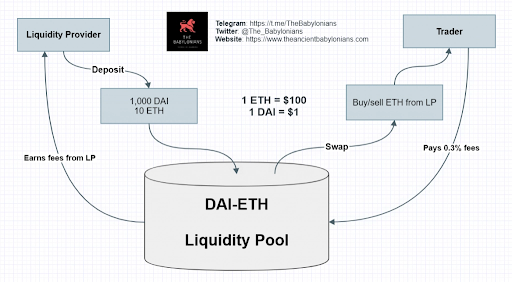
\includegraphics[scale=.75]{../misc/liquidityPool.png}

\caption{Illustration of General protocol structure}
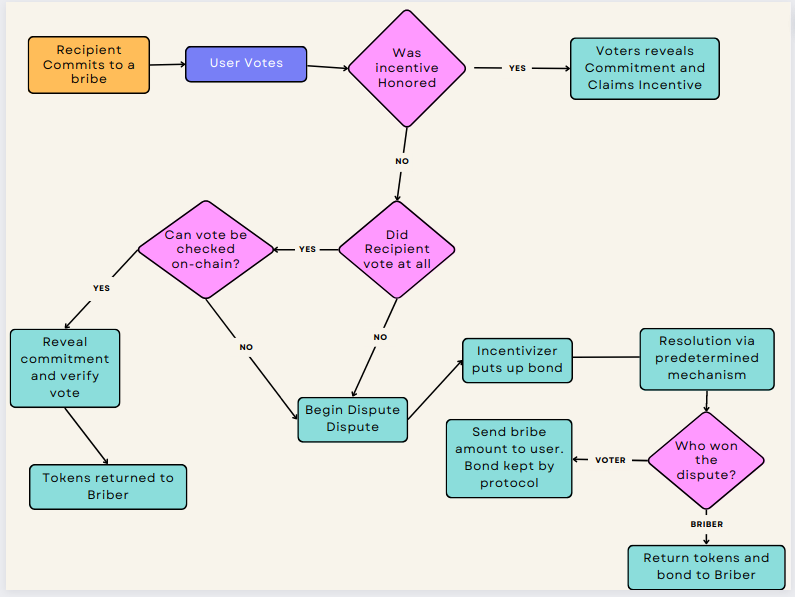
\includegraphics[scale=0.47]{../misc/protocol_structure.png}
\end{figure}

\newpage
\begin{figure}[p]
\centering
\caption{Workflow when an incentive IS honored}
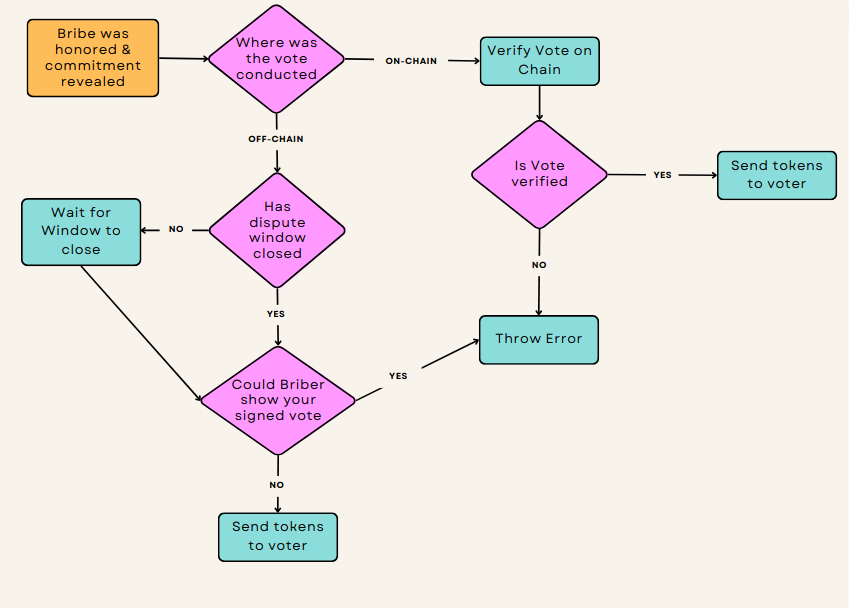
\includegraphics[scale=0.433]{../misc/reveal_structure.png}

\centering
\caption{Workflow when an incentive is NOT honored}
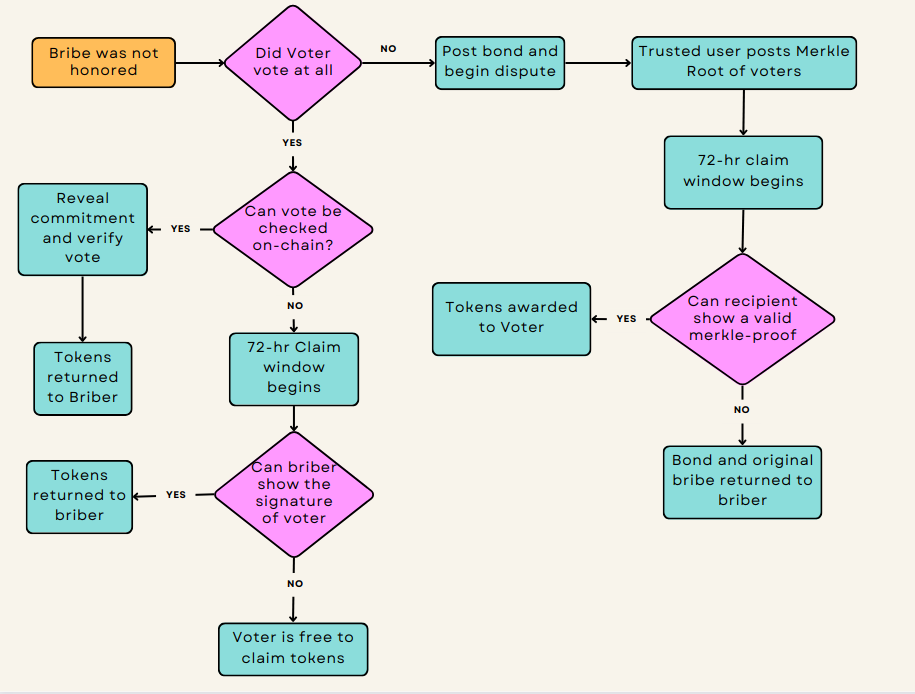
\includegraphics[scale=0.4]{../misc/claiming_userflow.png}
\end{figure}

\newpage
\begin{figure}[p]
\centering
\caption{Example Depiction of how price relates to quantity of users on each side of an incentive}
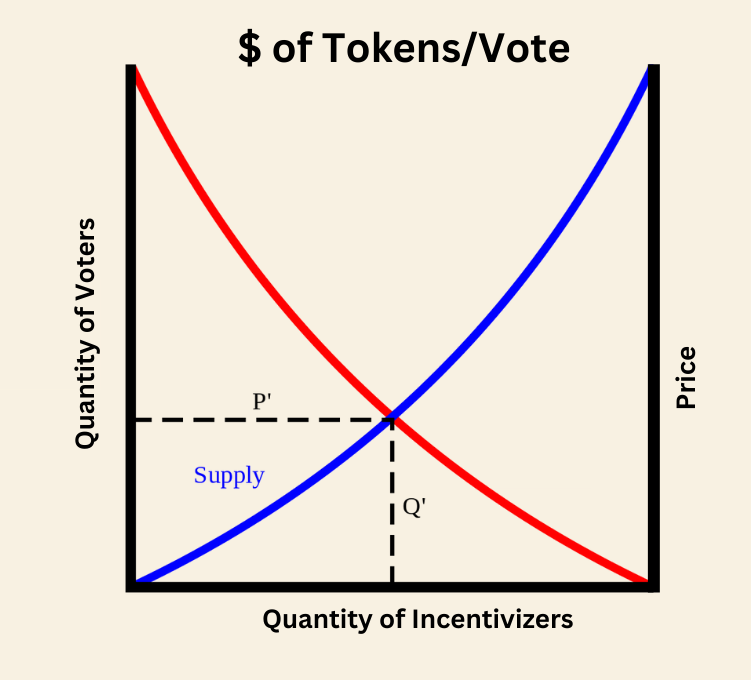
\includegraphics[scale=0.35]{../misc/supplyDemand.png}

\caption{Graph of Provided Liquidity for the \$MIM token over time}
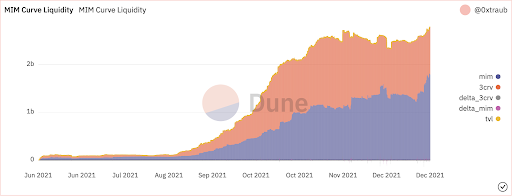
\includegraphics[scale=.8]{../misc/liquidity.png}
\end{figure}



\end{document}